%
% $RCSfile: graphical_user_interface.tex,v $
%
% Copyright (c) 2002-2007. Christian Heller. All rights reserved.
%
% Permission is granted to copy, distribute and/or modify this document
% under the terms of the GNU Free Documentation License, Version 1.1 or
% any later version published by the Free Software Foundation; with no
% Invariant Sections, with no Front-Cover Texts and with no Back-Cover
% Texts. A copy of the license is included in the section entitled
% "GNU Free Documentation License".
%
% http://www.cybop.net
% - Cybernetics Oriented Programming -
%
% Version: $Revision: 1.1 $ $Date: 2007-07-17 20:02:36 $ $Author: christian $
% Authors: Christian Heller <christian.heller@tuxtax.de>
%

\subsection{Graphical User Interface}
\label{graphical_user_interface_heading}
\index{Graphical User Interface}

A \emph{Graphical User Interface} (GUI) is mostly based on so-called graphical
\emph{Windows} which may overlap, or be ordered side-by-side on a screen.
Figure \ref{graphical_user_interface_figure} illustrates a typical GUI.

\begin{figure}[ht]
    \begin{center}
%        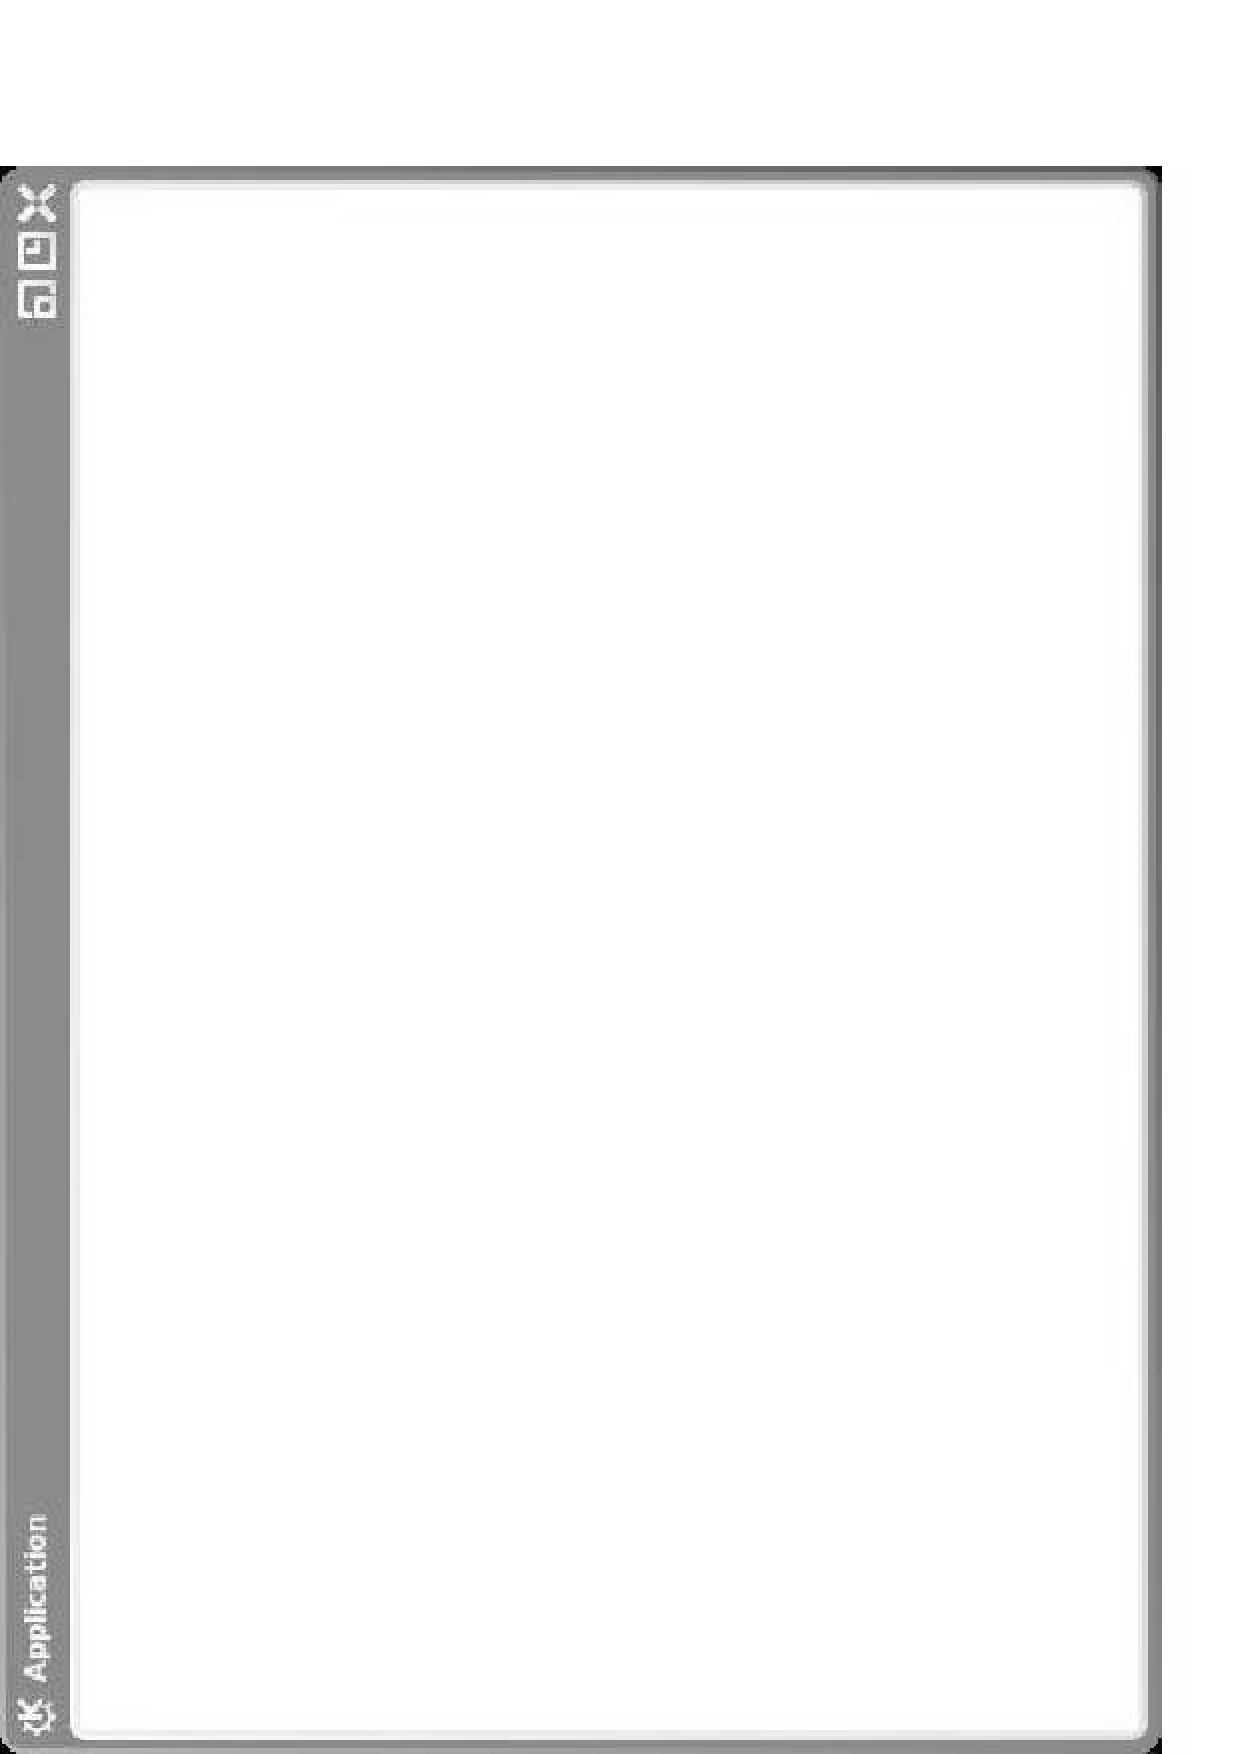
\includegraphics[scale=0.3,angle=-90]{graphics/graphical_user_interface.pdf}
        \caption{Graphical User Interface}
        \label{graphical_user_interface_figure}
    \end{center}
\end{figure}

\subsubsection{Shape Property}

\emph{required}

name=\texttt{'shape'}\\
abstraction=\texttt{'character'}\\
model=\texttt{'rectangle' \vline\ 'circle' \vline\ 'polygon'}

This property specifies the geometrical shape of the GUI.

\subsubsection{Layout Property}

\emph{required}

name=\texttt{'layout'}\\
abstraction=\texttt{'character'}\\
model=\texttt{'root' \vline\ 'coordinates' \vline\ 'compass'}

This property specifies the kind of layout of the GUI.

\subsubsection{Cell Property}

\emph{optional}, only if \emph{layout} property is \emph{compass}

name=\texttt{'cell'}\\
abstraction=\texttt{'character'}\\
model=\texttt{'north' \vline\ 'south' \vline\ 'west' \vline\ 'east' \vline\ 'centre'}

This property specifies the cell ordering, if \emph{compass} layout is used.

\subsubsection{Position Property}

\emph{required}

name=\texttt{'position'}\\
abstraction=\texttt{'integer'}\\
model=\texttt{x, y, z coordinates}

This property specifies the GUI element's origin.

\subsubsection{Size Property}

\emph{required}

name=\texttt{'size'}\\
abstraction=\texttt{'integer'}\\
model=\texttt{x, y, z extensions}

This property specifies the GUI element's extension.

\subsubsection{Background Property}

\emph{optional}

name=\texttt{'background'}\\
abstraction=\texttt{'character'}\\
model=\texttt{'black' \vline\ 'red' \vline\ 'green' \vline\ 'yellow' \vline\ 'blue' \vline\ 'magenta' \vline\ 'cobalt' \vline\ 'white'}

This property specifies the background colour of the GUI.

\subsubsection{Foreground Property}

\emph{optional}

name=\texttt{'foreground'}\\
abstraction=\texttt{'character'}\\
model=\texttt{'black' \vline\ 'red' \vline\ 'green' \vline\ 'yellow' \vline\ 'blue' \vline\ 'magenta' \vline\ 'cobalt' \vline\ 'white'}

This property specifies the foreground colour of the GUI.

\subsubsection{Title Property}

\emph{optional}, only if \emph{layout} property is \emph{root}

name=\texttt{'title'}\\
abstraction=\texttt{'character'}\\
model=\texttt{window title}

This property specifies the GUI element's (window's) title.

\subsubsection{Icon Property}

\emph{optional}, only if \emph{layout} property is \emph{root}

name=\texttt{'icon'}\\
abstraction=\texttt{'bmp' \vline\ 'jpeg' \vline\ 'png' \vline\ 'gif' \vline\ etc.}\\
model=\texttt{graphic file}

This property specifies the GUI element's (window's) icon.

\subsubsection{Expose Property}

\emph{optional}, only if GUI element should react to expose event

name=\texttt{'expose'}\\
abstraction=\texttt{'knowledge' \vline\ 'encapsulated'}\\
model=\texttt{logic knowledge model}

This property specifies the logic knowledge model to be executed if the GUI
element is exposed, for example shown again after having been hidden before.

\subsubsection{Mouse Over Property}

\emph{optional}, only if GUI element should react to mouse event

name=\texttt{'mouse\_over'}\\
abstraction=\texttt{'knowledge' \vline\ 'encapsulated'}\\
model=\texttt{logic knowledge model}

This property specifies the logic knowledge model to be executed if the mouse
is moved over the GUI element.

\subsubsection{Mouse Wheel Property}

\emph{optional}, only if GUI element should react to mouse event

name=\texttt{'mouse\_wheel'}\\
abstraction=\texttt{'knowledge' \vline\ 'encapsulated'}\\
model=\texttt{logic knowledge model}

This property specifies the logic knowledge model to be executed if the mouse
wheel is scrolled while the mouse pointer is over the GUI element.

\subsubsection{Left Press Property}

\emph{optional}, only if GUI element should react to mouse event

name=\texttt{'left\_press'}\\
abstraction=\texttt{'knowledge' \vline\ 'encapsulated'}\\
model=\texttt{logic knowledge model}

This property specifies the logic knowledge model to be executed if the left
mouse button is pressed.

\subsubsection{Left Release Property}

\emph{optional}, only if GUI element should react to mouse event

name=\texttt{'left\_release'}\\
abstraction=\texttt{'knowledge' \vline\ 'encapsulated'}\\
model=\texttt{logic knowledge model}

This property specifies the logic knowledge model to be executed if the left
mouse button is released.

\subsubsection{Left Click Property}

\emph{optional}, only if GUI element should react to mouse event

name=\texttt{'left\_click'}\\
abstraction=\texttt{'knowledge' \vline\ 'encapsulated'}\\
model=\texttt{logic knowledge model}

This property specifies the logic knowledge model to be executed if the left
mouse button is clicked. A mouse click is the combination of a mouse press- and
release event.
